\section{Classifiers overview} \label{classifiers}

Given that the main objective we want to reach with this section is to identify the best suited classifier for packed malware detection, it makes sense not to rush on one algorithm but rather consider a larger diversity of candidates to open up the field of possibilities. That's why it has been decided to start from the analysis of 7 different families of well-known classifiers, each containing sometimes more than one classifier. Let's briefly go through them to understand how they work.

\subsection{K-Nearest Neighbors} \label{KNN}

Probably one of the most popular and easy-to-understand algorithm in machine learning. We could think of this classifier as a model which stores every input data as a point on a plan. Each point holds its corresponding label. When given a brand new input, it will find the closest point in the plan in terms of Euclidean distance and associates it with the corresponding label. The \textbf{K} prefix in its name stands for the number of closest neighbors that should be considered when classifying. If set to a value higher than 1, a majority vote is used, meaning that the label with the highest frequency among all neighbors is chosen as the prediction for the new data point. An example is shown at figure \ref{fig:KNN} with two classes - green and blue - where the new data point will be assigned the color green according to the majority vote.

\begin{figure}[!ht]
\centering
  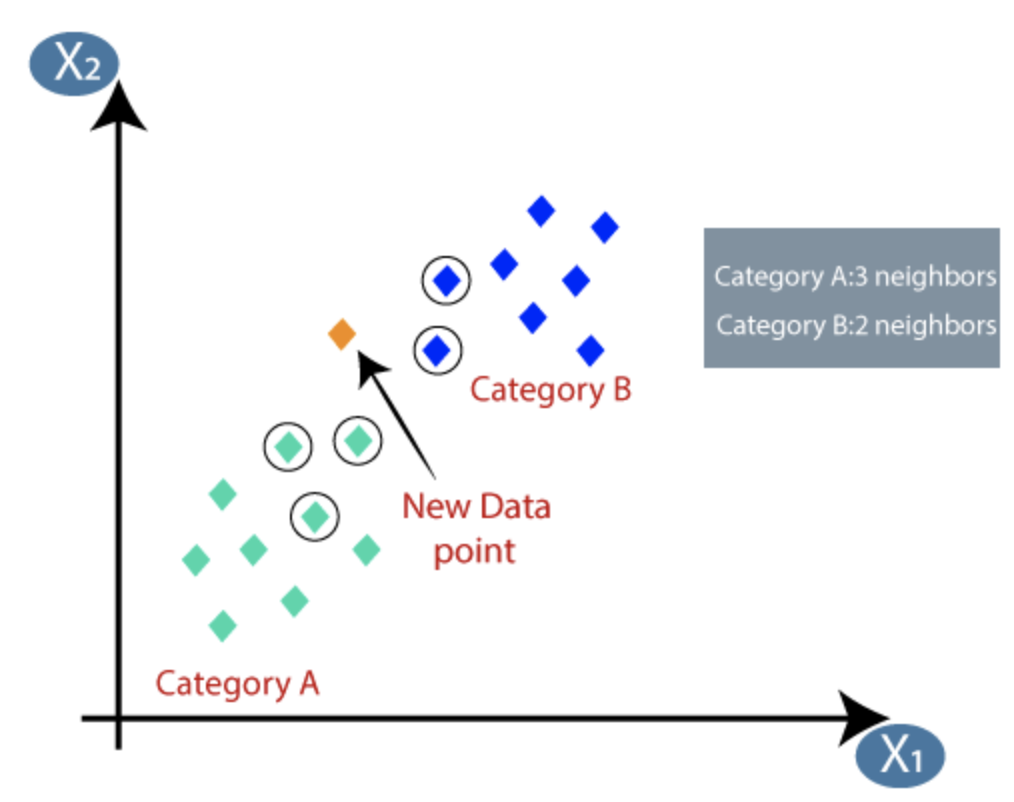
\includegraphics[width=0.80\linewidth]{Figures/KNN.png}
  \caption{Binary classification using the 5-Nearest Neighbors classifier \cite{java_knn}}
  \label{fig:KNN}
\end{figure}

The main strengths of this model lies in its ease of understanding and how fast it can provid good initial outcomes without a lot of adjustments. On the other side, when the number of samples and features grow intensively, predictions become really slow. It also requires preprocessing beforehand. KNN is therefore a good starting point before tackling more complex algorithms.

\subsection{Naive Bayes Classifiers}

This family of algorithm is known for being pretty fast when learning over a training set but sometimes at the cost of efficiency, as we will see later. Naive Bayes classifiers are probabilistic models based on the Bayes theorem:
$$ P(A \mid B) = \frac{P(B \mid A) \, P(A)}{P(B)} $$
The \textit{Naive} term comes from the fact that it is assumed that each feature is independent from another in the dataset. In other words, the model looks at each feature individually and collects simple statistics for each of them. Although this assumption of independence doesn't generalise well in real-world situations, it is accepted that it works well in practice.

We distinguish two classifiers among this family: the \textit{Gaussian} and the \textit{Bernoulli} Naive Bayes classifiers. Each of them differs in the distribution they use as their name indicates, the Gaussian distribution referring to the Normal distribution. While the first one can be applied to any continuous data, the Bernoulli distribution assumes binary data. The reason why we chose these two distributions was to compare whether using only binary values could be more efficient than sticking to continuous data. Officially, the Naive Bayes classifier family also embeds a third classifier, which uses the Multinomial distribution. We decided not to consider it because such distribution assumes count data, meaning that each feature has to represent an integer sum of something. This classifier is more suited for occurrence problems, like counting how often words appear in a text, rather than for binary classification.

\subsection{Linear Models} \label{LM}

The main concept behind linear models for classification is the use of a linear function of the form 
\[y = x[1] * w[1] + x[2] * w[2] + ... + x[p] * w[p] + b \]
where \textit{x} is the set of feature values of length \textit{p}, \textit{w} and \textit{b} are parameters learned by the model, respectively the weights and the y-axis offset, and \textit{y} is the prediction. Since this work is a matter of binary classification, the predicted value is thresholded at zero. A value of \textit{y} greater than zero corresponds to class 0 while a value smaller than zero belongs to class 1. Therefore, the decision boundary could be represented as a line or a plane that separates the data in two classes.

Linear models is a very large family and embeds various linear algorithms. They all differ in the way they produce the parameters and which kind of regularisation they use, knowing they also offer a lot of parameters tuning. We decided to stick to the two most common linear classification algorithms, namely \textit{linear support vector machines} and \textit{logistic regression}. Logistic regression finds a model which maximises the conditional likelihood of the training data using Sigmoid functions while linear support vector machine maximises the margin between points closest to the classification boundary - see figure \ref{fig:LM}. They also have different loss functions, but we will come back to that later in the test phase.

\begin{figure}[ht]
\centering
    \begin{minipage}[b]{0.43\linewidth}
    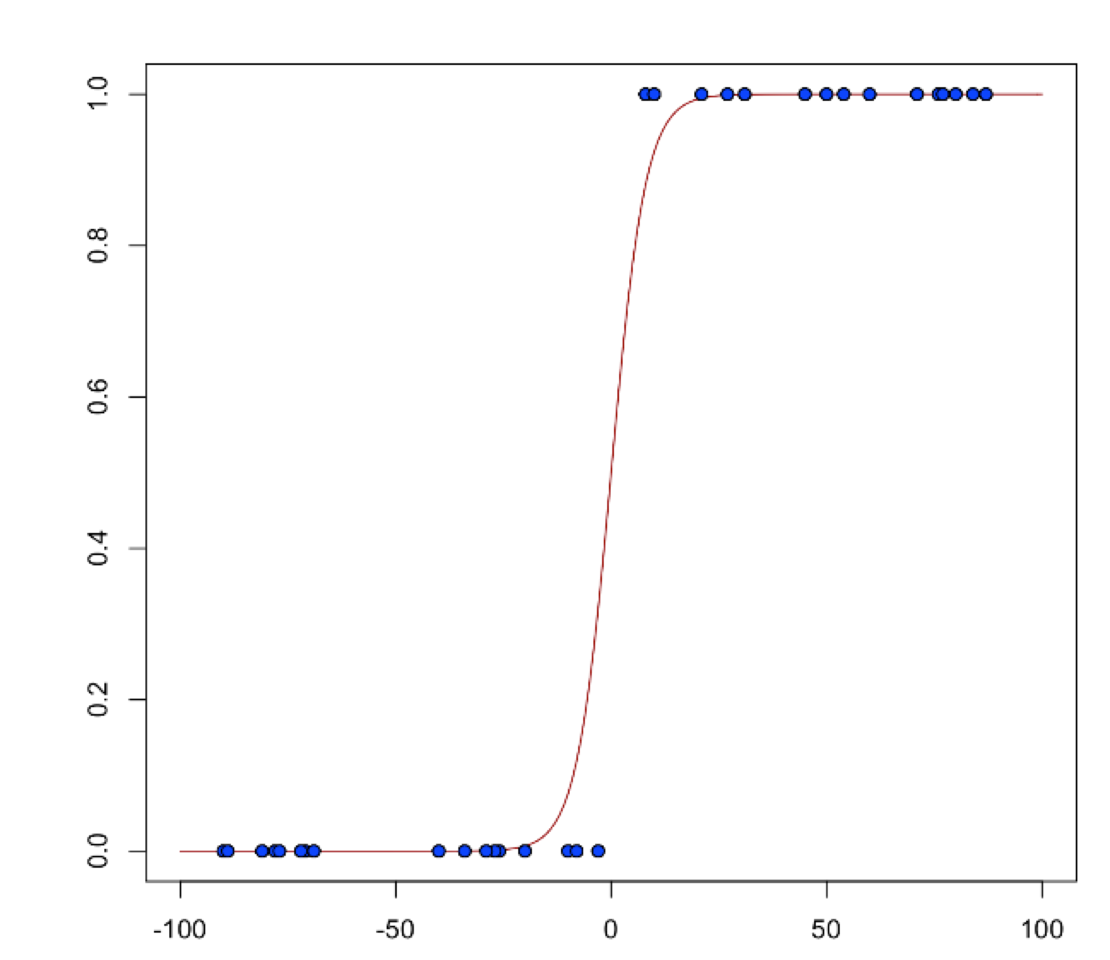
\includegraphics[width=\linewidth]{Figures/LM1.png}
\end{minipage}
\quad
\begin{minipage}[b]{0.52\linewidth}
    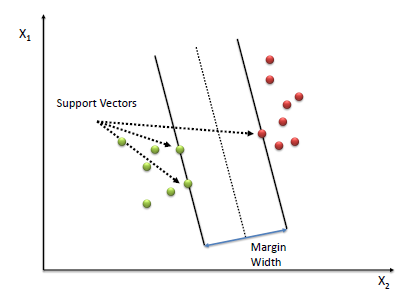
\includegraphics[width=\linewidth]{Figures/LM2.png}
\end{minipage}
\captionsetup{justification=centering}
\caption{Logistic regression (left) \cite{logreg1} \\ and linear support vector machine (right) \cite{logreg2}}
\label{fig:LM}
\end{figure}

Linear models are particularly fast to train and predict and have the property to scale up to thousands of samples.

\subsection{Decision Trees}

Decision trees, as their names suggest, can be seen as trees where each branch is the answer to an \textit{if/else statement}, with the decisions at the leaves, such as in figure \ref{fig:DT}. In the procedure of building the decision tree, all features are considered. Different combinations of splits are tested and the best match is selected using a specific cost function. Therefore, it is    straightforward to guess that the more features we have, the biggest the tree becomes. Feature relevance and feature selection will therefore be of huge concern in the following experiments. Decision trees also offer several tools to reduce complexity and overfitting \footnote{Overfitting means that the model produces a learning which is too close to the training set and doesn't generalize well on the test set, but these notions will be more deeply explained when proceeding to the experiments.} like pruning or depth limitation.

\begin{figure}[!ht]
  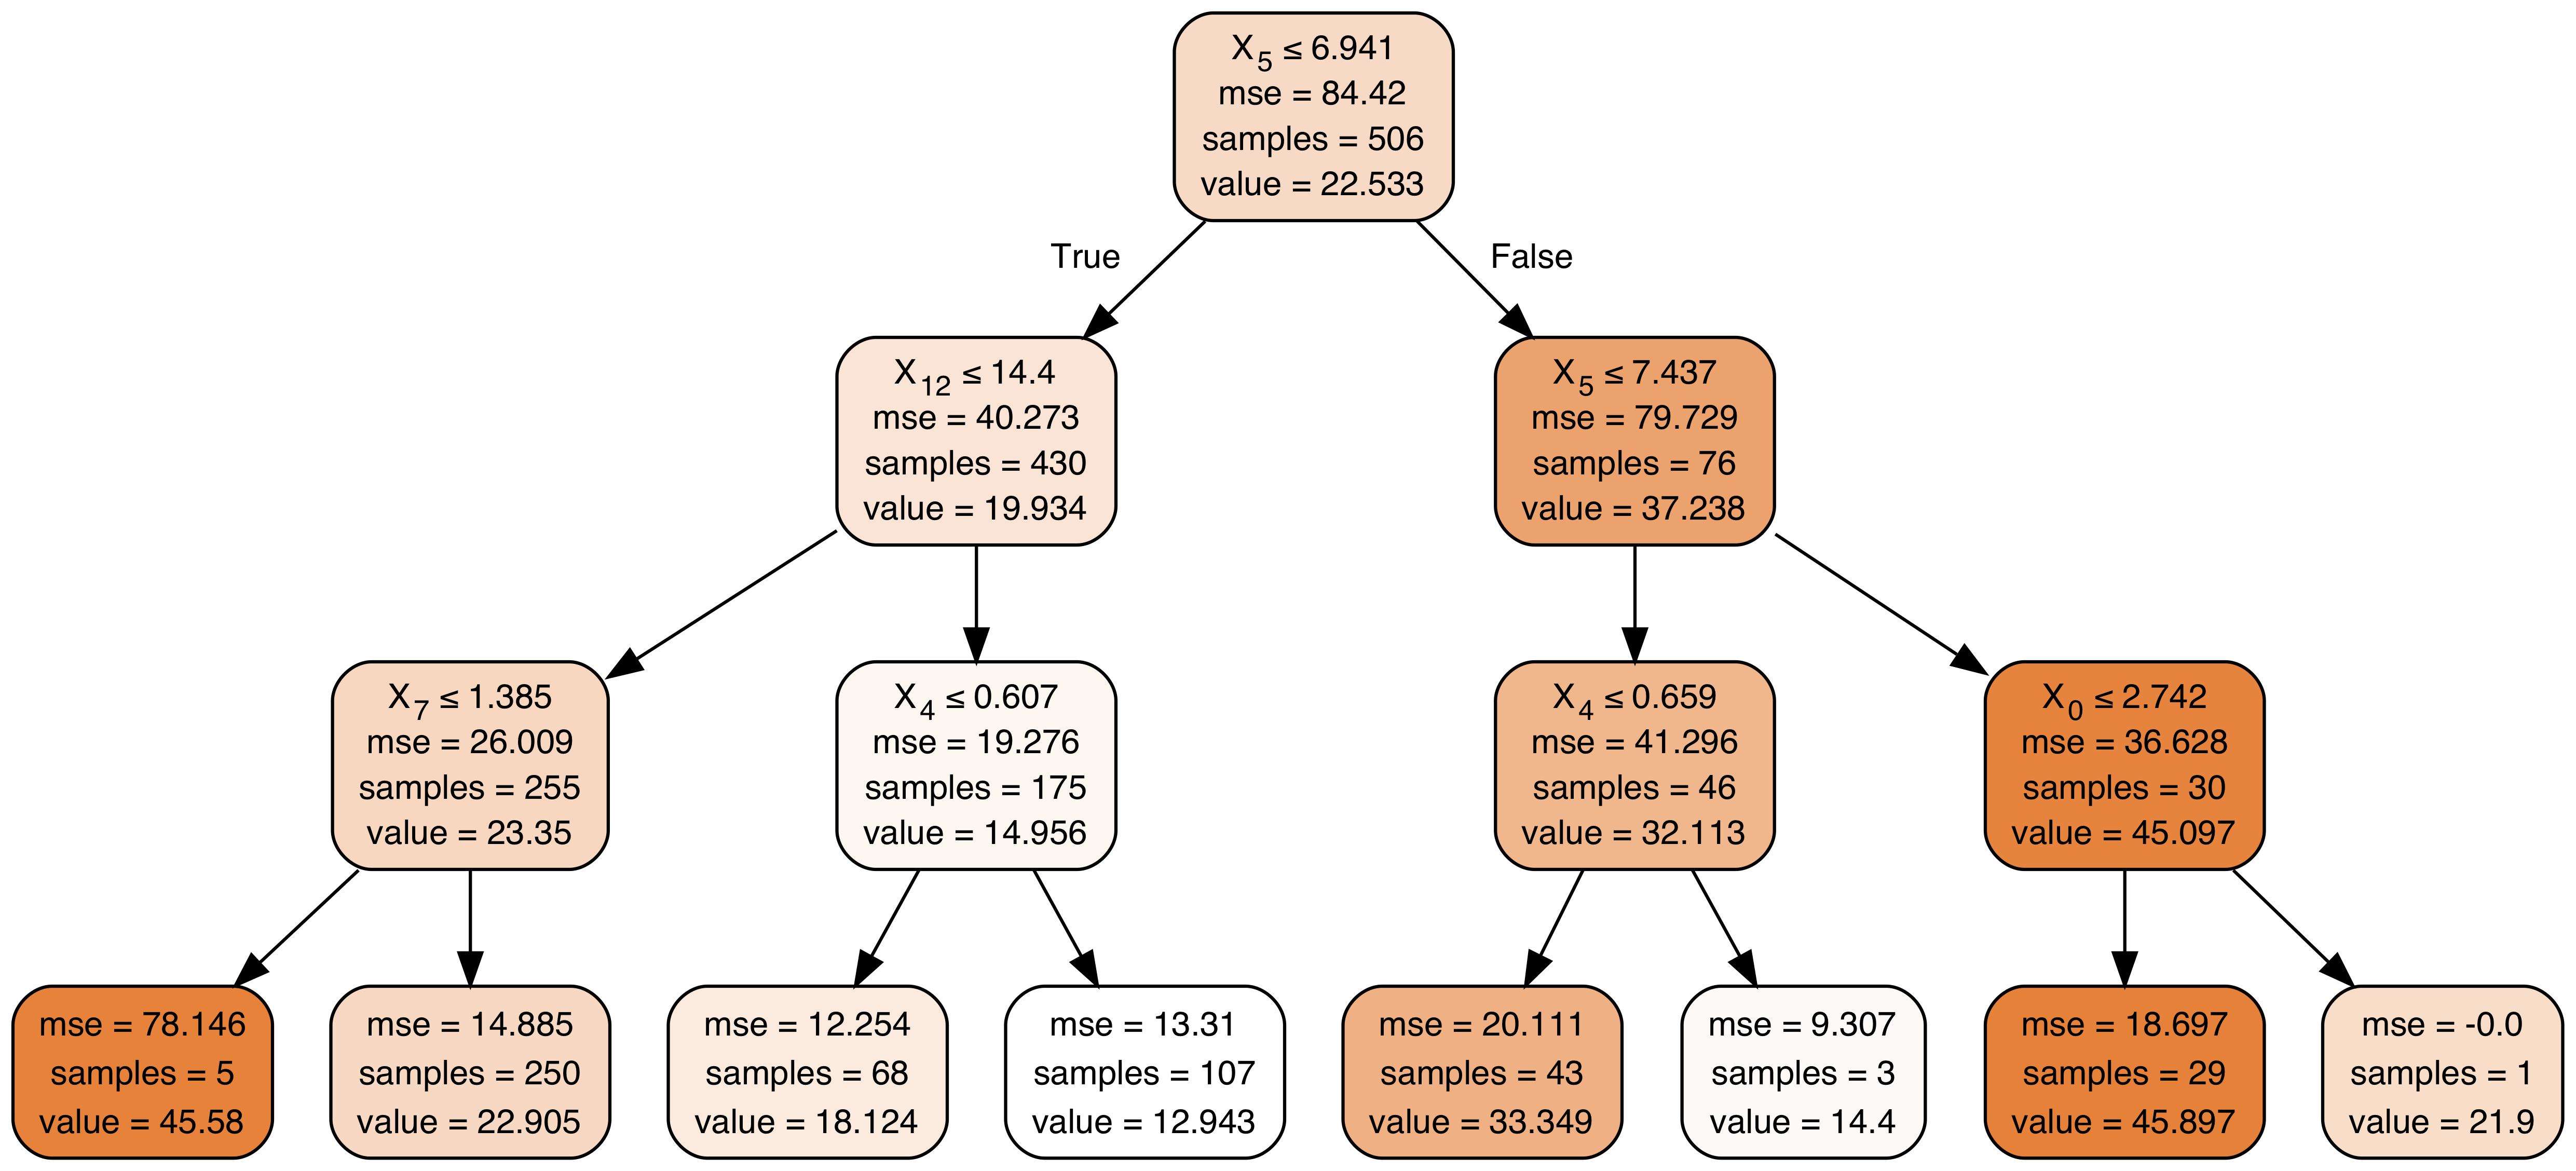
\includegraphics[width=\linewidth]{Figures/DT.png}
  \caption{Example of a simple decision tree \cite{dt_source}}
  \label{fig:DT}
\end{figure}

In addition to the traditional model, another version of decision tree is also considered in this work, namely DL8.5 \cite{DL8.5}, which only works with binary data. This implementation is an improvement of classical decision trees in the sense that it uses a cache of itemsets combined with branch-and-bound search in order to create less complex trees and avoid unnecessary computations. Since it is said to provide better performance than any competing methods, comparing it with the other classifiers is in our interest.

Decision trees are widely used in machine learning because they give really good outcomes without the need to prepare the data extensively. Indeed, each feature is processed separately and the splits are independent of the number of samples. Moreover, they support the mixture of both binary and continuous data.

\subsection{Ensemble of Decision Trees}

This category gathers algorithms that are built on the combination of multiple machine learning models, in this case namely decision trees. The raise of such classifiers is due to the wish of solving variance and bias that single decision trees might suffer of. The main idea is to combine many weak learners to shape a stronger one. We distinguish two major classifiers that have been proved to perform particularly well on a wide range of datasets: \textit{Random Forests} and \textit{Gradient Boosted Decision Trees}. Note that while combining several decision trees is indeed more efficient, it implies more resource consumption and computation power.

Random Forests is basically the combination of slightly different decision trees. While a single tree might do a great job at predicting, it could also be overfitting on part of the data. Random Forests therefore address this issue by averaging the results of several decision trees, resulting in a globally reduced overfitting while keeping the predictive power of each tree. The \textit{random} nature of this algorithm resides in the creation of the decision trees, which are built upon a randomly generated set of samples and features, keeping the best split. Each tree is then trained individually before aggregation with its peers. Figure \ref{fig:RF} illustrates the key principle of Random Forests.

\begin{figure}[!ht]
  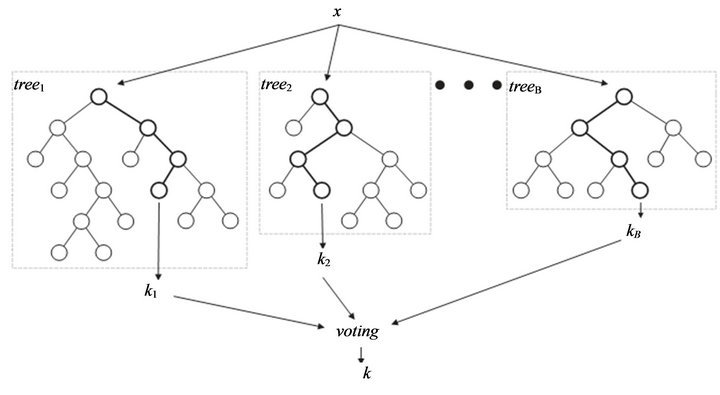
\includegraphics[width=\linewidth]{Figures/RF.png}
  \caption{Example of a Random Forest composed of \textit{B} decision trees \cite{edt_source}}
  \label{fig:RF}
\end{figure}

Gradient Boosted Decision Trees work by using a technique called \textit{Boosting} while Random Forests use \textit{Bagging}. This process is serial in the sense that it creates one tree after another, each tree trying to correct the errors of the previous one. The idea is to start with very shallow trees, often called \textit{weak learners}, which provide good prediction only on some parts of the data. More and more trees are then added to iteratively increase the global performance by reducing the loss margin. The main advantage of Gradient Boosted Decision Trees over Random Forests is that since they use very shallow trees, the model is more economical in terms of memory. On the other hand, they tend to be harder to tune than Random Forests.

\subsection{Kernelized Support Vector Machines}

Also referred to as SVM, they are an extension of Linear Models. They allow for more complex models that can be defined using hyper-planes, which is nothing but the three-dimensional version of a line that separates the data points in two classes - in the case of binary classification. The math behind the construction of this hyper-plane is quite out of scope for this work, especially as in this respect, \texttt{scikit-learn} offers a high level of abstraction. The \textit{kernelized} aspect refers to the Kernel trick used by the SVM to convert any low dimensional space into a higher one by using a set of functions like polynomial, Gaussian, Sigmoid, etc ... \textit{Support vectors} stands for the idea of keeping only relevant points to construct the decision boundary, namely the ones that lie on the border between the two classes. Figure \ref{fig:SVM} illustrates the transformation from a 2D (left) to 3D plane (right).

\begin{figure}[ht]
\centering
    \begin{minipage}[b]{0.485\linewidth}
    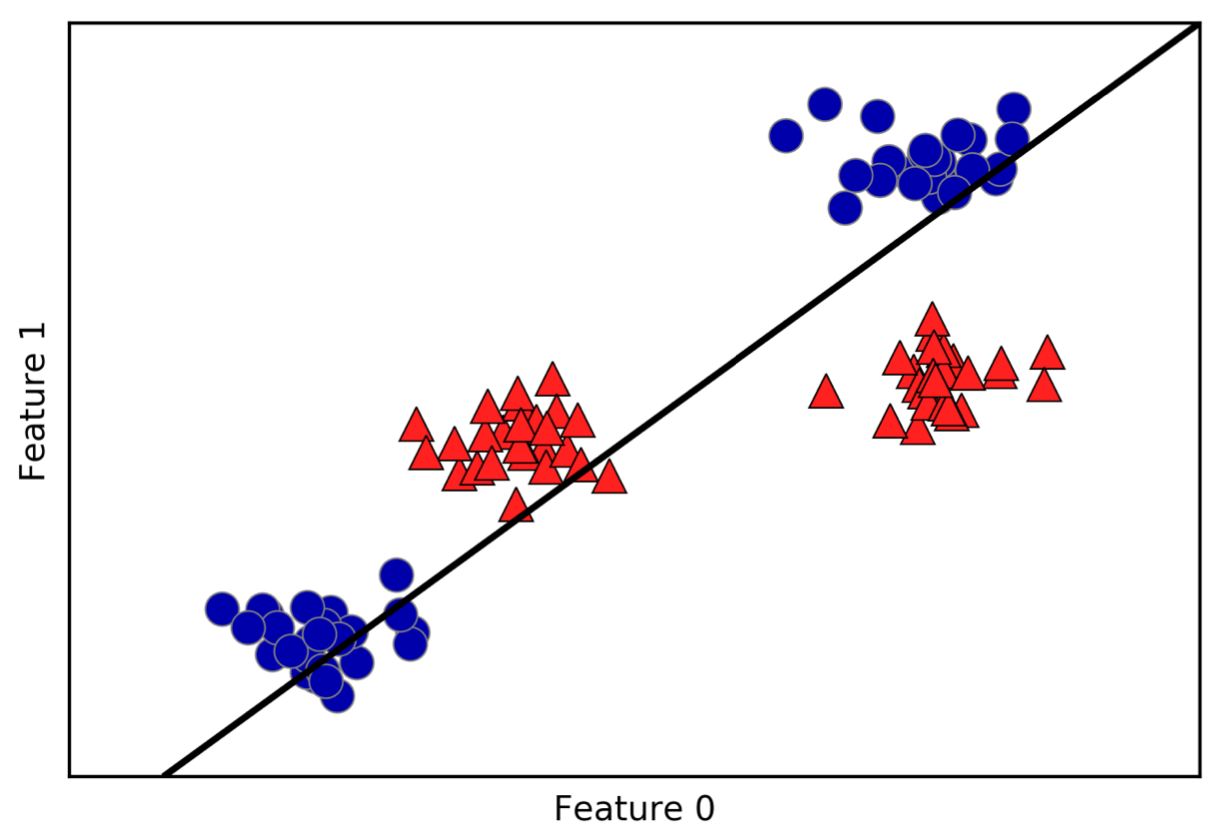
\includegraphics[width=\linewidth]{Figures/SVM1.png}
\end{minipage}
\quad
\begin{minipage}[b]{0.45\linewidth}
    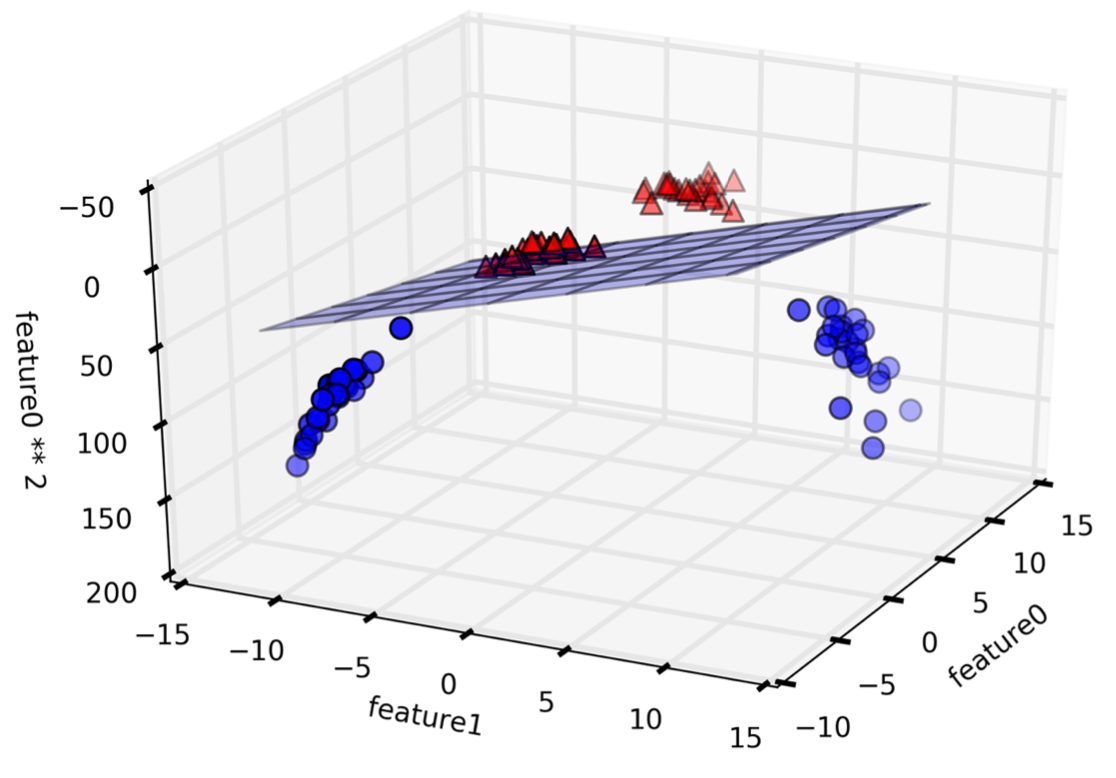
\includegraphics[width=\linewidth]{Figures/SVM2.png}
\end{minipage}
\caption{Decision boundary found by LinearSVM (left) and by SVM (right) \cite{ML}}
\label{fig:SVM}
\end{figure}

While SVM work well on a variety of datasets, they are known to suffer from performance degradation when scaled to a large number of samples. It will therefore be interesting to observe how they behave with our datasets. They perform really well on features that represent measurements in similar units and of the same scale, meaning that pre-processing is also an important step in its learning process.

\subsection{Neural Networks}

Mainly used in Deep Learning, Neural Networks reckon thousands of different classifiers suited for specific uses. One of the most popular is certainly the Multi-Layer Perceptrons - hereafter MLP - algorithm. It can be viewed as a generalization of linear models that are comprised of one or more layers of neurons. Remember the equation of linear models
\[y = x[0] * w[0] + w[1] * x[1] + ... + w[p] * x[p] + b \]
where \textit{y} is the weighted sum of the input features in \textit{x} by the coefficients in \textit{w}. With MLP, this process of weighted sums is repeated multiple times. Data is fed to the input layer, then there may be one or more hidden layers representing intermediate processing steps, and eventually predictions are made on the output layer. The number of coefficients to learn is therefore significantly increased. But the thing is that, mathematically speaking, computing multiple weighted sums is the same as deriving just one. What MLP provides then is the use of an additional nonlinear function, applied to the weighted sum of each hidden unit. This new value is then used in the weighted sum that computes the final \textit{y} - see figure \ref{fig:MLP}.

\begin{figure}[!ht]
\centering
  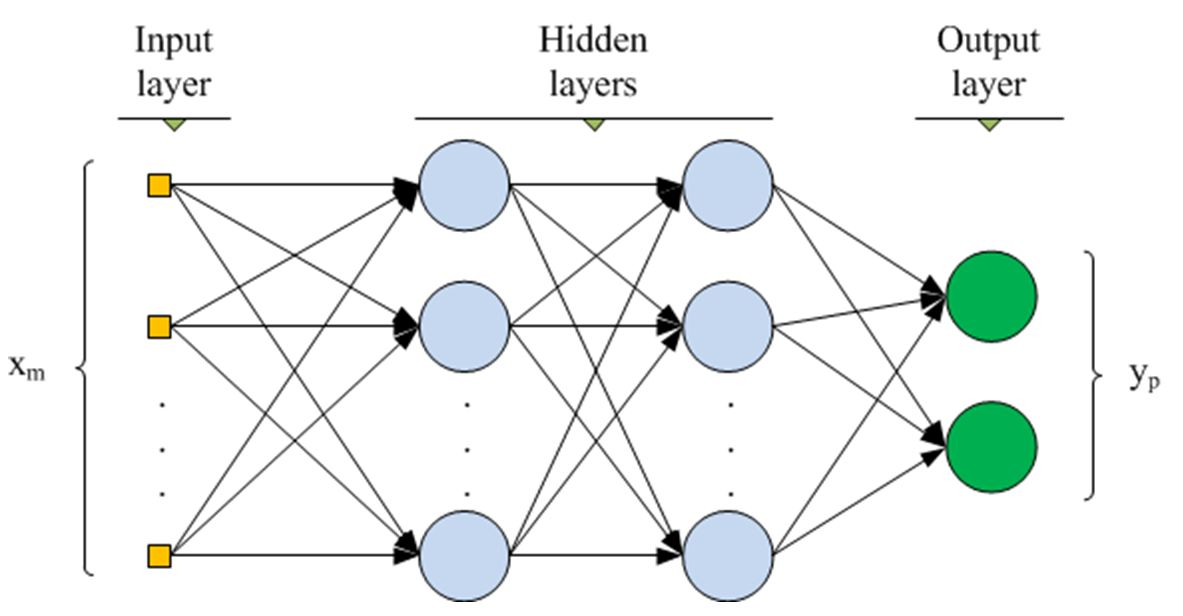
\includegraphics[width=0.80\linewidth]{Figures/MLP.jpg}
  \caption{Multi-Layer Perceptron with two hidden layers \cite{mlp_source}}
  \label{fig:MLP}
\end{figure}

The main advantage of using Neural Networks is that they have shown their efficiency to deal with large datasets and come up with incredibly complex models, as opposed to SVM. But has one could have guessed, this is done at the cost of a really long training time, precise pre-processing and wise parameters tuning, as for SVM. In the hypothesis of unlimited resources, Neural Networks are often unbeatable.